\documentclass[9pt, handout]{beamer}

%!TEX root = ../notas_de_clase.tex

%preamble

%language
\usepackage[spanish,es-nodecimaldot]{babel}
\usepackage[utf8]{inputenc}
\usepackage{apacite}
\usepackage[absolute,overlay]{textpos}

%packages
\usepackage[Algoritmo]{algorithm}
\usepackage{algorithmicx}
\usepackage[noend]{algpseudocode}
\usepackage{mathtools}
\setlength {\marginparwidth}{2cm}
\usepackage{todonotes}
\usepackage{amsbsy}
\usepackage{amssymb}
\usepackage{amsmath,bm}
\usepackage{dsfont}

\usepackage{xcolor}
\providecommand{\sred}[1]{\textcolor{red}{#1}}
\providecommand{\sblue}[1]{\textcolor{blue}{#1}}
\providecommand{\red}[1]{\textcolor{red}{\text{#1}}}
\providecommand{\blue}[1]{\textcolor{blue}{\text{#1}}}
\providecommand{\redb}[1]{\textcolor{red}{\textbf{#1}}}
\providecommand{\blueb}[1]{\textcolor{blue}{\textbf{#1}}}
\usepackage{graphicx}
\usepackage{fancybox}
\usepackage{booktabs}
\usepackage{caption}
\usepackage{float}
%\usepackage[longend,ruled,algochapter,linesnumbered,lined,boxed,commentsnumbered,spanish]{algorithm2e}
%\usepackage[algo2e]{algorithm2e}
\usepackage{amssymb}
\usepackage{amstext}
\usepackage{bm}
\usepackage{wrapfig}
\usepackage{subcaption} % para_unsupervised_chapter

%formatting

\usepackage[export]{adjustbox}

%caption para figuras
\captionsetup[figure]{width=.8\linewidth, font=small,labelfont={bf},name={Fig.},labelsep=period}
\captionsetup[table]{width=.8\linewidth,font=small,labelfont={bf},name={Tabla},labelsep=period}



\ifx\byn\undefined
    \definecolor{my_blue}{HTML}{C2D5FF}
    \definecolor{my_red}{HTML}{FFC2C2}
    \definecolor{my_yellow}{HTML}{FFFFE0}
\else
    \definecolor{my_blue}{HTML}{FFFFFF}
    \definecolor{my_red}{HTML}{FFFFFF}
    \definecolor{my_yellow}{HTML}{FFFFFF}
\fi


\usepackage[framemethod=TikZ]{mdframed}
\mdfdefinestyle{discusion}{%
    %linecolor=black,
    %outerlinewidth=0pt,
    roundcorner=0pt,
    innertopmargin=5pt,
    innerbottommargin=5pt,
    innerrightmargin=20pt,
    innerleftmargin=20pt,
    backgroundcolor=my_blue}

\colorlet{Green}{green!90}


\mdfdefinestyle{ejemplo}{%
    %linecolor=black,
    %outerlinewidth=0pt,
    roundcorner=0pt,
    innertopmargin=5pt,
    innerbottommargin=5pt,
    innerrightmargin=20pt,
    innerleftmargin=20pt,
    backgroundcolor=my_yellow}


\mdfdefinestyle{pendiente}{%
    style = discusion, 
    backgroundcolor=my_red}


\RequirePackage{url}



%definitions
\def\td{{\text d}}
\def\cN{{\mathcal N}}
\def\cX{{\mathcal X}} 
\def\cC{{\mathcal C}} 
\def\N{{\mathbb N}}
\def\d{{\text d}}
\def\datos{{\mathcal D}}
\def\eye{{\mathbb I}}
\def\ssum{{\scriptstyle\sum}}
\def\bepsilon{{\bm \epsilon}}
\def\tx{\tilde{x}}
\def\tX{\tilde{X}}
\def\thetaMAP{\theta_\text{MAP}}
\newcommand{\gp}{\ensuremath{\mathcal{GP}}}
\newcommand{\pr}{\ensuremath{\mathbb{P}}}
\newcommand{\x}{\ensuremath{\mathbf{x}}}
\newcommand{\z}{\ensuremath{\mathbf{z}}}
\newcommand{\cvector}{\ensuremath{\mathbf{c}}}
\newcommand{\e}{\ensuremath{\mathbf{e}}}
\newcommand{\y}{\ensuremath{\mathbf{y}}}
\newcommand{\bx}{\ensuremath{\textcolor{blue}{X}}}
\newcommand{\by}{\ensuremath{\textcolor{blue}{Y}}}
\newcommand{\rx}{\ensuremath{\textcolor{red}{X_*}}}

\newcommand{\R}{\mathbb{R}}
\newcommand{\norm}[1]{\left\lVert#1\right\rVert}




\DeclareMathOperator*{\argmax}{arg\,max}
\DeclareMathOperator*{\argmin}{arg\,min}
\DeclareMathOperator{\E}{\mathbb{E}}
\DeclareMathOperator{\V}{\mathbb{V}}
\DeclareMathOperator{\KL}{\text{KL}}
\DeclareMathOperator{\MVN}{\text{MVN}}
\newcommand\deq{\stackrel{\mathclap{\normalfont\mbox{\tiny def}}}{=}}
%\newcommand{\E}[1]{\mathbb E \left[#1\right]}
\newcommand{\trace}[1]{\text{Tr} \left[#1\right]}


\usepackage{amsthm}

%-------------------------------------------
% Newtheorem
%-------------------------------------------
\newtheorem{axioma}{\textcolor{red}{Axioma}}
\newtheorem{definicion}{Definición}
\newtheorem*{notacion}{Notación}
\newtheorem{teorema}{Teorema}
\newtheorem{corolario}{Corolario}
\newtheorem{lema}{Lema}
\newtheorem{lemaZ}{\textcolor{red}{Lema}}
\newtheorem{propiedad}{Propiedad:}
\newtheorem{proposicion}{Proposición:}
\newtheorem*{observacion}{Observación}
\newtheorem*{comentario}{Comentario}
\newtheorem*{ejemplo}{Ejemplo}
\newtheorem*{resultado}{Resultado}
\newtheorem*{propuesto}{Ejercicio propuesto}
\newtheorem*{demostracion}{Demostración} % No se usa, usar \begin{proof}\end{proof} que son por default.

%listing paackage para código
\usepackage{listings}
\usepackage{xcolor}
 
\definecolor{codegreen}{rgb}{0,0.6,0}
\definecolor{codegray}{rgb}{0.5,0.5,0.5}
\definecolor{codepurple}{rgb}{0.58,0,0.82}
\definecolor{backcolour}{rgb}{0.95,0.95,0.92}
 
\lstdefinestyle{mystyle}{
    xleftmargin=0.15\textwidth,
    linewidth=0.8\textwidth,
    backgroundcolor=\color{backcolour},   
    commentstyle=\color{codegreen},
    keywordstyle=\color{magenta},
    numberstyle=\tiny\color{codegray},
    stringstyle=\color{codepurple},
    basicstyle=\ttfamily\footnotesize,
    breakatwhitespace=true,         
    breaklines=true,                 
    captionpos=b,                    
    keepspaces=true,                 
    numbers=left,                    
    numbersep=5pt,                  
    showspaces=false,                
    showstringspaces=false,
    showtabs=false,                  
    tabsize=2
}
 
\lstset{style=mystyle}

\numberwithin{equation}{section}

\usetheme{simple}

\title{Clase 6: Inferencia bayesiana (parte 2)}
\subtitle{MA5204 Aprendizaje de Máquinas}
\date{\today}
\author{Felipe Tobar} 
\titlegraphic{
\begin{figure}[htp] 
    \centering
        
\includegraphics[width=0.15\textwidth]{../img/Uchile.pdf}% 
\end{figure}
}
\institute{Department of Mathematical Engineering \&\\ Center for Mathematical Modelling\\Universidad de Chile}

\begin{document}
\begin{frame}
  \titlepage
\end{frame}

%Recuerdo.
\begin{frame}{Recuerdo}
Se vio que el enfoque bayesiano estaba basado en la relación dada por el teorema de Bayes
	\begin{equation*}
	p(\theta|x) = \frac{p(x|\theta)p(\theta)}{p(x)} \propto p(x|\theta)p(\theta),\label{eq:Bayes}
\end{equation*}
donde $p(\theta)$ era el prior sobre el parámetro $\theta$ y contenía el conocimiento experto.\\~\ \pause

Además, se estableció que un prior $p(\theta)$ es \emph{conjugado} a la verosimilitud $p(D|\theta)$, cuando la posterior $p(\theta|D)$ está en la misma familia que el prior $p(\theta)$.\\~\ \pause

Se estudió el caso del modelo gaussiano, donde se llegó a la siguiente conclusión:

\begin{itemize}
	\item \textbf{$\mu$ desconocido y $\sigma^2$ conocido:} el prior gaussiano para $\mu$ es conjugado con la verosimilitud gaussiana.
	\item \textbf{$\sigma^2$ desconocido y $\mu$ conocido:} el prior gamma-inverso para $\sigma^2$ es conjugado con la verosimilitud gaussiana. 
\end{itemize}

\end{frame}

%prior conjugado: modelo lineal gaussiano.
\begin{frame}{Prior conjugado para el modelo lineal gaussiano}
\framesubtitle{(regresón bayesiana)}

Para un conjunto de observaciones $\datos=\{(x_i,y_i)\}_{i=1}^n$, el modelo de regresión lineal puede ser escrito en forma vectorial utilizando la matriz de diseño trabajada en el capítulo de regresión:
\begin{equation*}
 	Y = \tX\theta + \bepsilon.
 \end{equation*} \pause
De esta forma, la verosimilitud está dada por 
\begin{align*}
	L(\theta,\sigma^2) &= \MVN(Y; \tX\theta, \eye\sigma^2)\\
					&\propto \left(\sigma^2\right)^{-n/2}   \exp\left(-\frac{1}{2\sigma^2} (Y - \tX\theta)^\top(Y - \tX\theta)\right).\nonumber
\end{align*} \pause
Esta última  expresión es proporcional a una distribución gamma-inversa para $\sigma^2$ y proporcional a una MVN para $\theta$. Consecuentemente, esta verosmilitud tiene los mismos priors conjugados que el modelo gaussiano vistos en la clase anterior. 
	
\end{frame}

%prior conjugado: modelo lineal gaussiano.
\begin{frame}{Prior conjugado para el modelo lineal gaussiano}
\framesubtitle{(regresón bayesiana)}


Consideremos el caso en que $\sigma^2$ es conocido, por lo que elegimos el prior gaussiano para $\theta$ dado por
\begin{equation*}
	p(\theta) \propto \exp\left(-\frac{1}{2\sigma^2}(\theta-\theta_0)^\top\Lambda_0(\theta-\theta_0)\right)
\end{equation*}\pause

Entonces, de forma análoga al caso gaussiano, se obtiene una distribución posterior \textbf{para el parámetro $\theta$ de la regresión lineal} dada por $\MVN(\theta; \theta_n,\sigma^2\Lambda_n^{-1})$, donde  
\begin{align*}
	\theta_n &= (\tX^\top \tX + \Lambda_0)^{-1} (\tX^\top  Y + \Lambda_0\theta_0) = (\tX^\top \tX + \Lambda_0)^{-1} (\tX^\top \tX (\tX^\top \tX)^{-1}\tX^\top  Y + \Lambda_0\theta_0)\label{eq:mean_post_lin_g}\\
	\Lambda_n &= (\tX^\top \tX + \Lambda_0)
\end{align*}\pause
Es decir:

\begin{itemize}
	\item La media posterior $\theta_n$ es un promedio ponderado entre la media a priori $\theta_0$ y el estimador de máxima verosimilitud $(\tX^\top \tX)^{-1}\tX^\top  Y$.
	\item La varianza $\Sigma_n = \Lambda_n^{-1}$ se mueve desde la varianza a priori $\Lambda_0^{-1}$ hacia $(\tX^\top \tX)^{-1}$ a medida recibimos más observaciones, resultando en un modelo más preciso.
\end{itemize}
	
\end{frame}

%prior conjugado: modelo lineal gaussiano (ejemplo).
\begin{frame}{Regresión linea bayesiana: ejemplo}

Implementación de la regresión lineal bayesiana, para $y = 2x-2	+ \epsilon$, con $\epsilon\sim\cN(0,0.5^2)$. 
	
	\begin{figure}[H]
	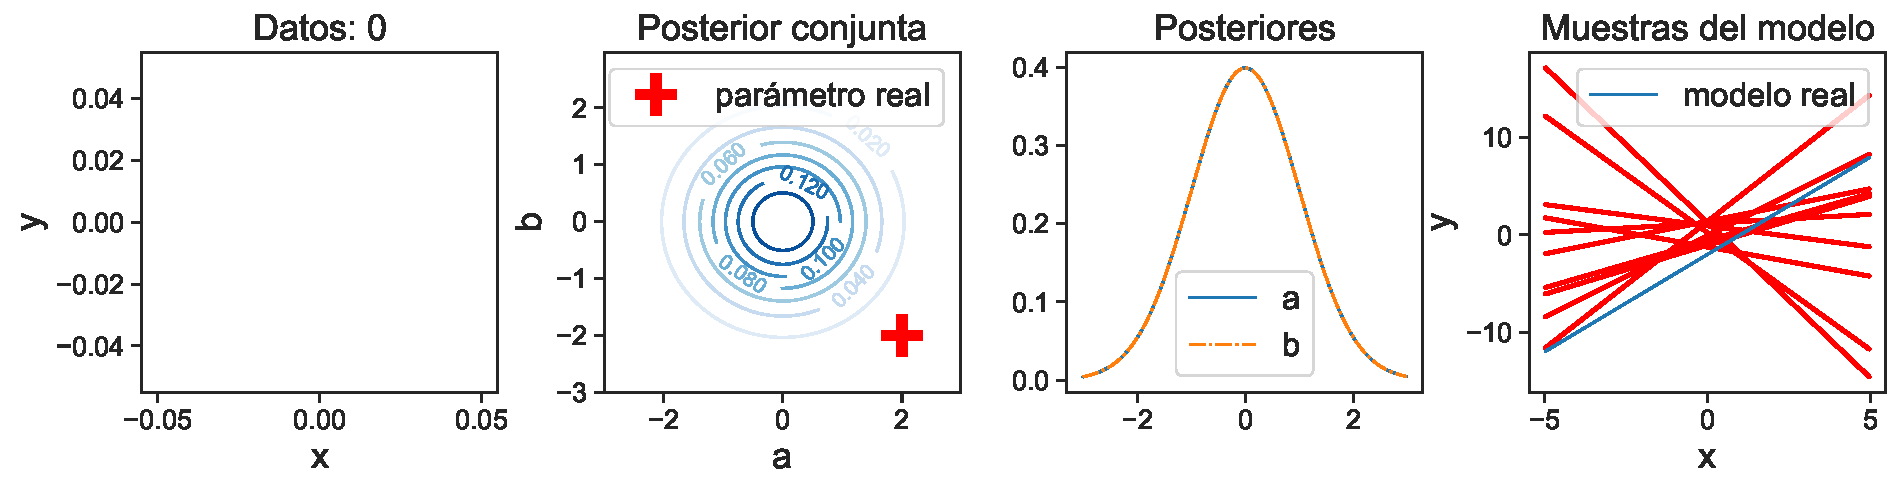
\includegraphics[height=0.25\textheight,frame]{../img/cap2_bayesian_lin_reg_0.pdf}\\
	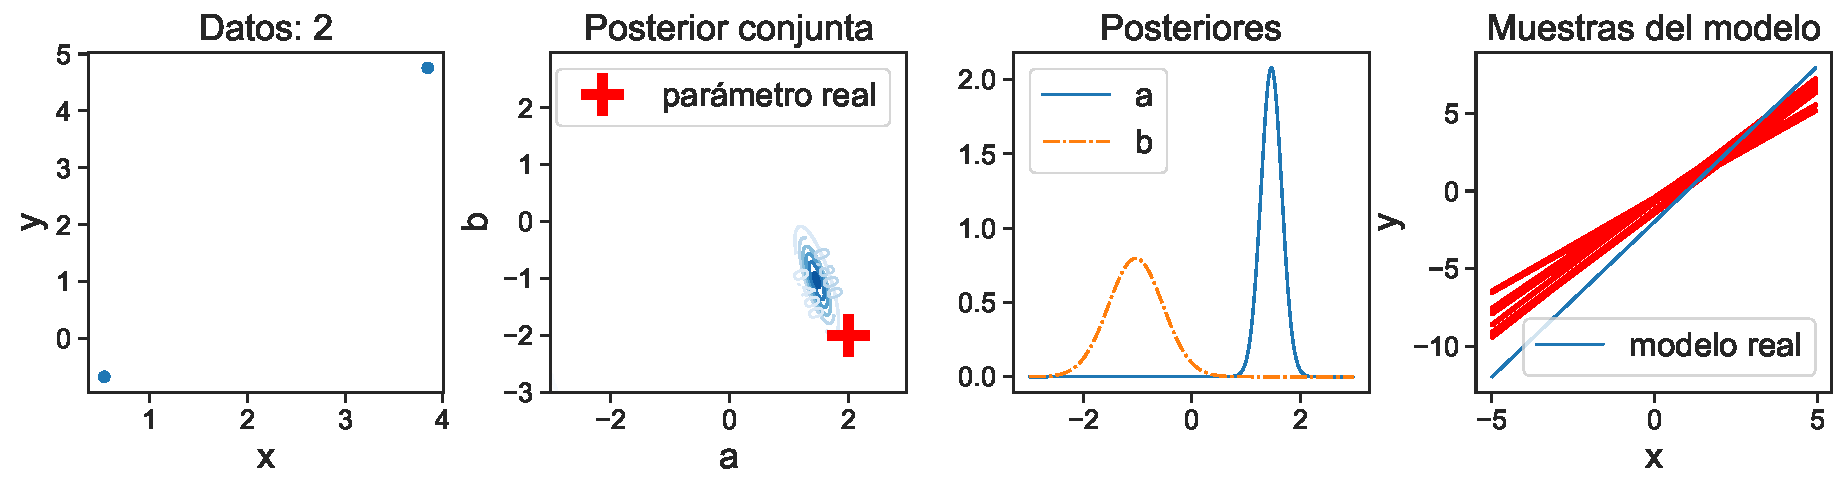
\includegraphics[height=0.25\textheight,frame]{../img/cap2_bayesian_lin_reg_2.pdf}\\
	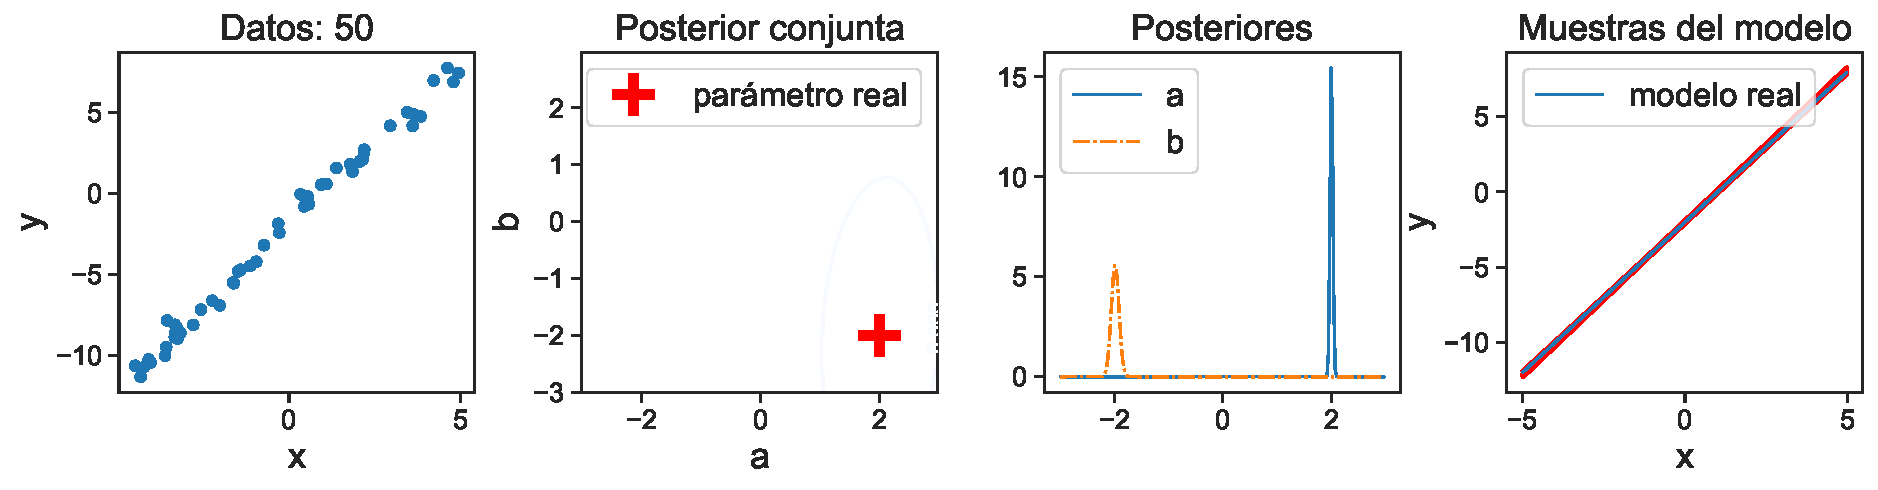
\includegraphics[height=0.25\textheight,frame]{../img/cap2_bayesian_lin_reg_50.pdf}
\end{figure}

\end{frame}

%Máximo a posteriori (MAP).
\begin{frame}{Máximo a posteriori (MAP)}

Existen distintas formas de extraer una estimación puntual de un parámetro $\theta$ a partir de la distribución posterior $p(\theta|\datos)$ como por ejemplo, la moda, media o mediana, los cuales son equivalentes cuando la posterior es gaussiana.\\~\ \pause

Siguiendo un criterio similar al de máxima verosimilitud consideraremos estimaciones puntuales mediante la maximización de la distribución posterior, resumiendo la información de la posterior mediante su moda. 

\begin{definition}[Máximo a posteriori]
Sea $\theta\in\Theta$ un parámetro con distribución posterior $p(\theta|\datos)$ definida en todo $\Theta$, entonces nos referimos a estimación puntal dada por
\begin{equation*}
	\thetaMAP = \argmax_{\Theta}p(\theta|\datos),
\end{equation*}
como \emph{máximo a posteriori (MAP)}.

\end{definition}\pause

La relación entre MAP y MV puede ser vista como un término adicional al momento de maximizar:
\begin{equation*}
	\thetaMAP = \argmax_{\theta\in\Theta}p(\theta|\datos) = \argmax_{\theta\in\Theta}p(\datos|\theta)p(\theta)= \argmax_{\theta\in\Theta}\left(\underbrace{\log p(\datos|\theta)}_{l(\theta)} + \log p(\theta)\right)
\end{equation*}
	
\end{frame}

%MAP para el modelo lineal gaussiano.
\begin{frame}{MAP para el modelo lineal gaussiano}

Para el modelo lineal y gaussiano, se puede considerar un prior gaussiano multivariado donde cada coordenada de $\theta$ tendrá un prior independiente de media cero y varianza $\sigma_\theta^2$.\\ \pause

Asumiendo la varianza del ruido $\sigma_\epsilon^2$ conocida, se puede calcular $\thetaMAP$ como:
\begin{align}
	\theta_\text{MAP}^\star 	&= \argmax_\theta p(Y|\tX,\theta)p(\theta)\nonumber\\
	&= \argmax_\theta \left(\prod_{i=1}^N \frac{1}{\sqrt{2\pi}\sigma_\epsilon} \exp\left[{\frac{-1}{2\sigma_\epsilon^2}(y_i-\theta^\top\tx_i)^2}\right]\right)									\frac{1}{(\sqrt{2\pi}\sigma_\theta)^{M+1}} \exp\left({\frac{-\theta^\top\theta}{2\sigma_\theta^2}}\right) \nonumber\\
	&= \argmax_\theta  \frac{1}{(\sqrt{2\pi}\sigma_\epsilon)^N} \frac{1}{(\sqrt{2\pi}\sigma_\theta)^{M+1}} \exp\left( \sum_{i=1}^N{\frac{-1}{2\sigma_\epsilon^2}(y_i-\theta^\top\tx_i)^2} -{\frac{||\theta||^2}{2\sigma_\theta^2}}\right) \nonumber\\
	&= \argmin_\theta \sum_{i=1}^N{(y_i-\theta^\top\tx_i)^2} +{\frac{\sigma_\epsilon^2}{\sigma_\theta^2}||\theta||^2}\nonumber
\end{align}\pause

Esta expresión es equivalente al funcional de ridge regression, es decir, la solución MAP del modelo lineal y gaussiano con prior gaussiano es equivalente a la de mínimos cuadrados regularizados con orden de  regularización $p=2$.\\

\end{frame}

%Consideraciones generales.
\begin{frame}{Consideraciones generales}

\begin{itemize}
	\item En el caso anterior, si se hubiese elegido un prior exponencial $p(\theta)\propto\exp(-\gamma|\theta|)$, se hubiese llegado llegado a MCR con regularización $p=1$ (LASSO).\pause
	\item Desde ahora, nos referirnos como MAP a \textbf{cualquier} estimación puntual, pues, como acabamos de ver, esta es equivalente a MCR y al mismo tiempo equivale al criterio de máxima verosimilitud cuando el prior es uniforme.\pause
	\item Para modelos generales (distintos al caso lineal y gaussiano) el MAP no podrá ser calculado de forma explícita imponiendo 
\begin{equation*}
 	\nabla_\theta  \log p(\theta|\datos) = 0,
 \end{equation*}
 sino que se tendrán que considerar algoritmos de optimización. En particular se utilizan algoritmos basados en derivadas con iteraciones de la forma
 \begin{equation*}
 	\theta_{i+1} = \theta_i + \eta \nabla_\theta  \log p(\theta_i|\datos), \label{eq:itera_MAP_grad}
 \end{equation*}
 donde se espera que la secuencia $\{\theta_i\}_{i\in\N}$ converja, es decir, $\nabla_\theta  \log p(\theta_i|\datos) \to 0$.
\end{itemize}

\end{frame}

\end{document}
